\section{Topologie}
\label{sec:RealisierungTopologie}
Nachdem in Kapitel \ref{sec:KonzeptionMeshNetz} ein Konzept für die Topologie entwickelt wurde folgt in diesem Unterkapitel die Beschreibung der Umsetzung des Mesh-Netzes, sowie der allgemeine Aufbau der gesamten Topologie. 
\subsection{Allgemeine Beschreibung}
Das gesamte Projekt des Sensorknoten lässt sich in fünf Ebenen unterteilen (siehe Grafik \ref{img:KonzeptionMeshNetz}). Im den folgenden Abschnitten werden diese vier Schichten genauer erläutert.
\begin{figure}
	\centering
	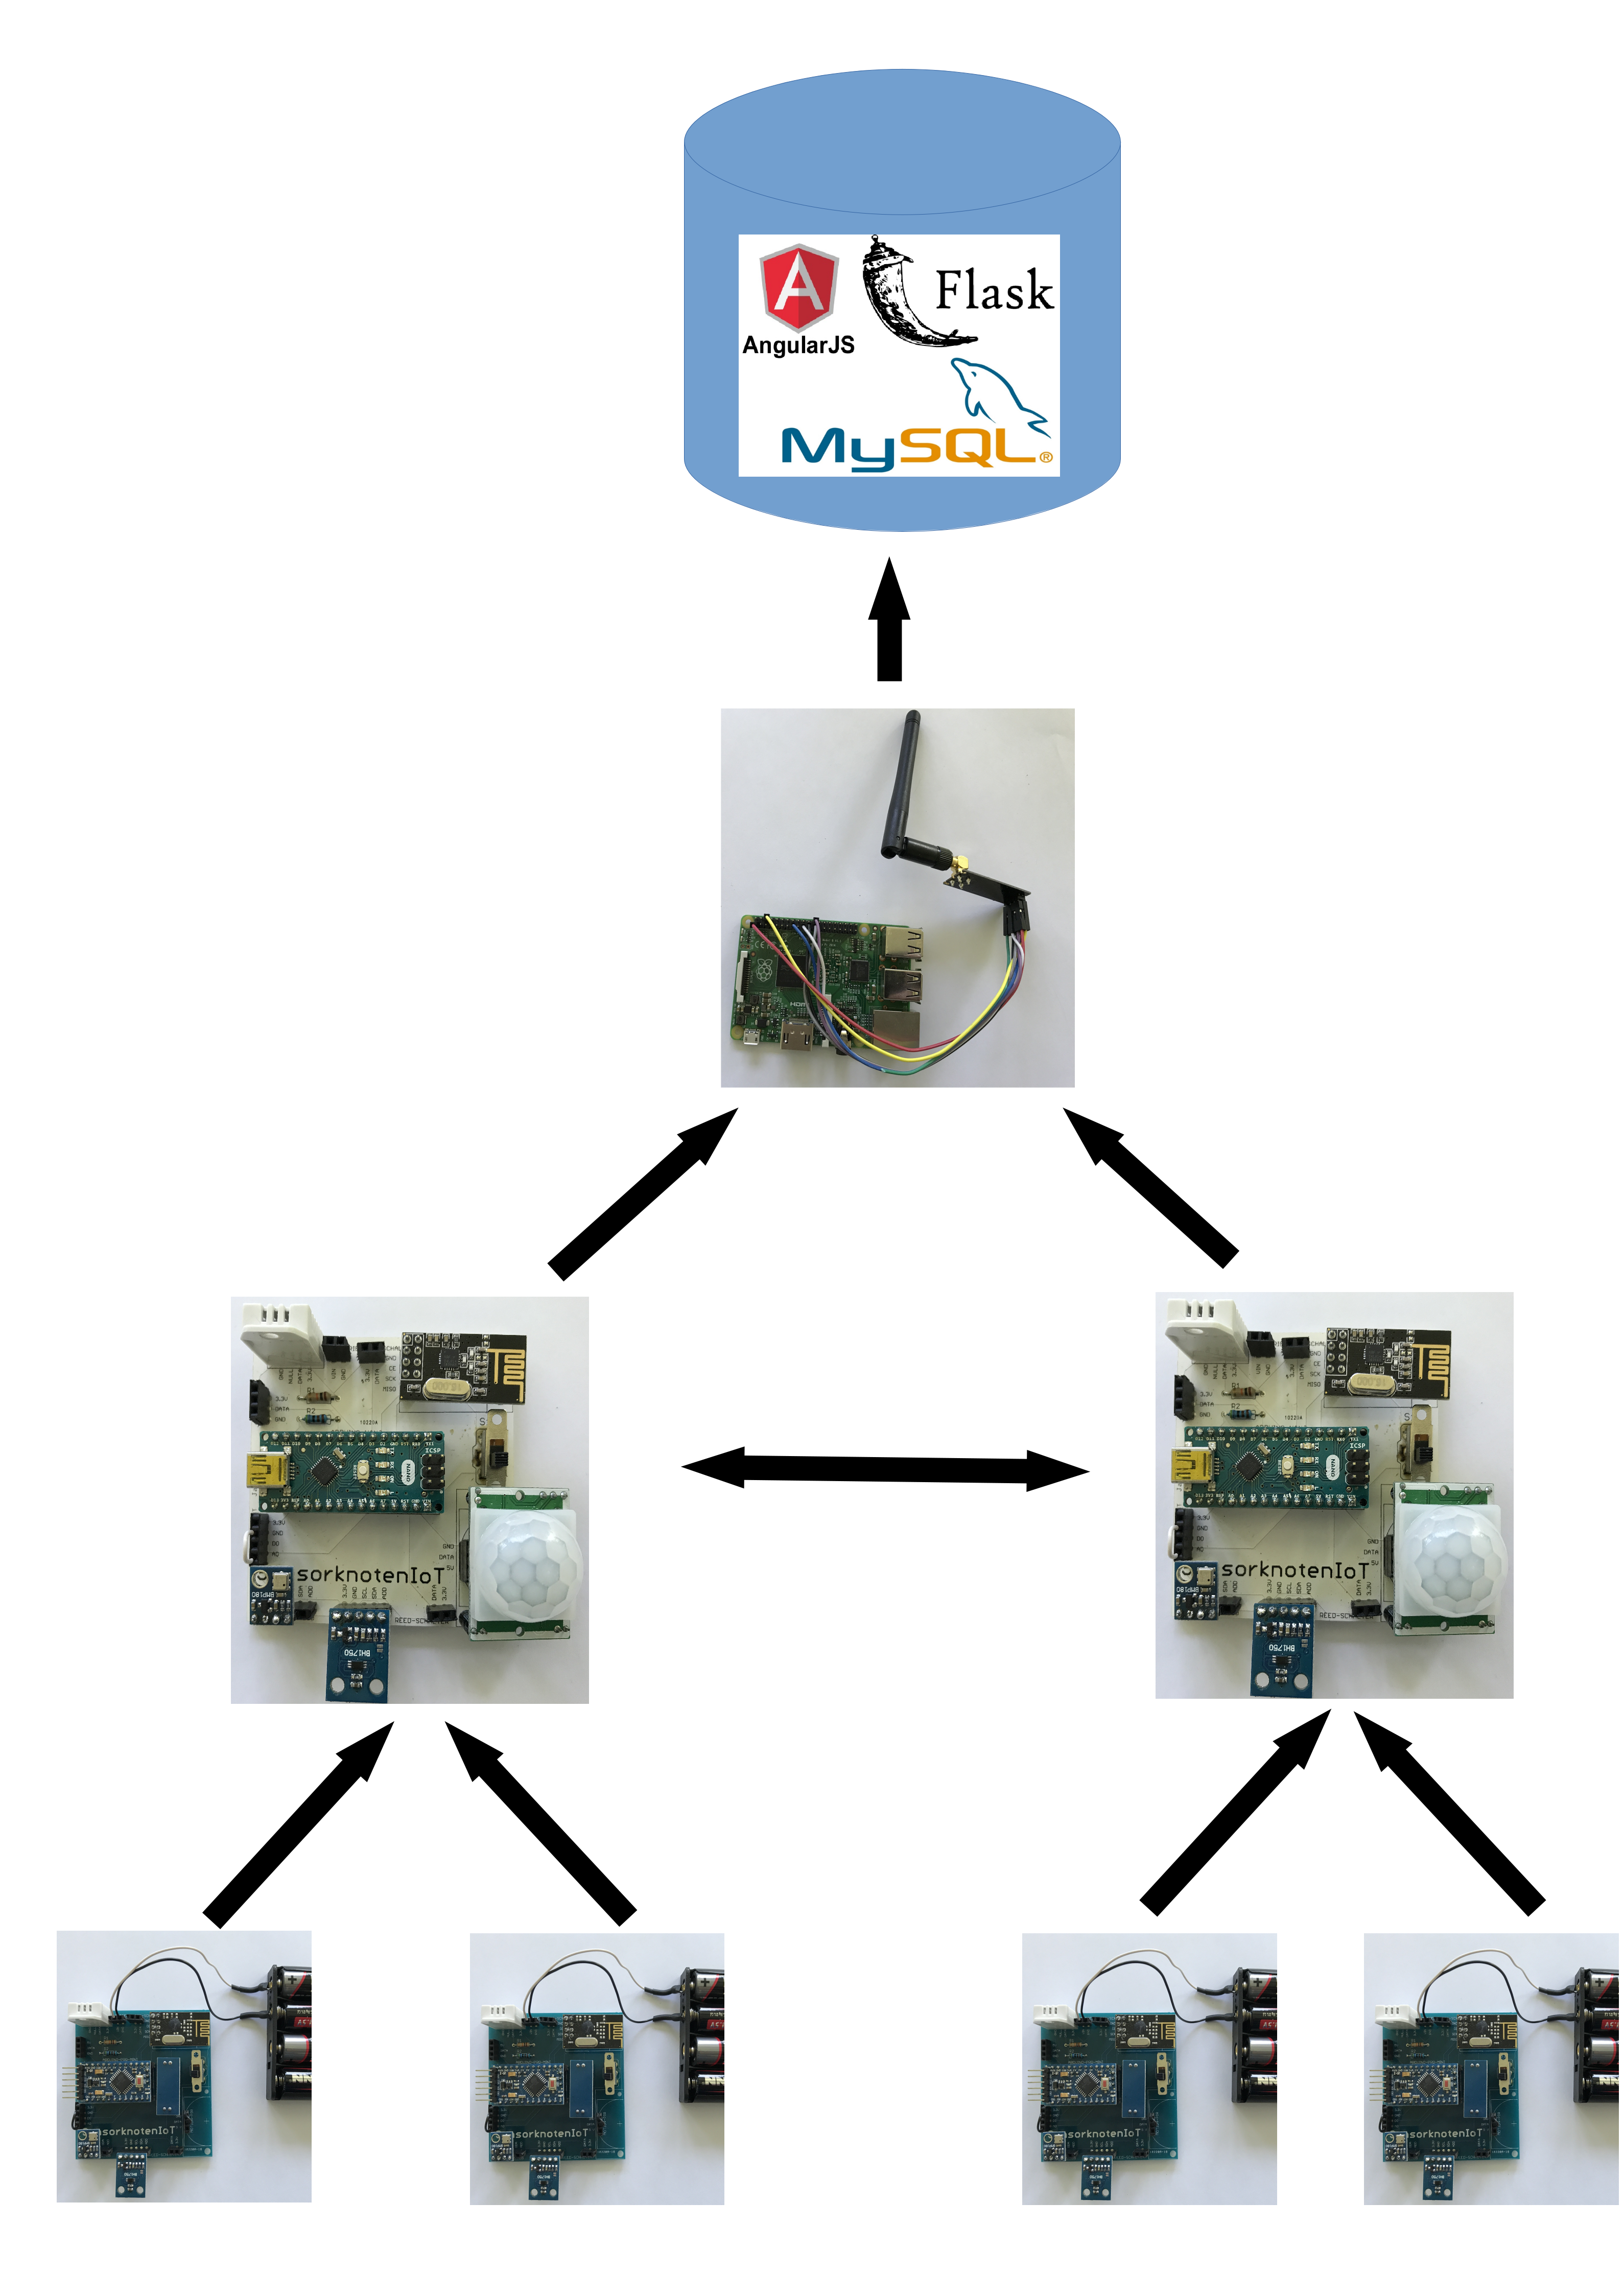
\includegraphics[width=0.6\textwidth]{bilder/topologie}
	\caption{Topologie Sensorknoten}
	\label{sec:KonzeptionMeshNetz}
\end{figure}
\paragraph{Energiesparender Sensorknoten} Der energiesparende Sensorknoten wurde mit einem Arduino Pro Mini realisiert. Dieser ist extrem energiesparend und übernimmt keinerlei Weiterleitungsfunktion im Mesh-Netz. Dieser Sensorknoten sendet seine Daten entweder direkt dem Raspberry Pi oder einem normalen Sensorknoten. Dieser leitet die  Nachricht dann zum Raspberry Pi weiter. Auf den genauen Aufbau des energiesparenden Sensorknoten wird in Kapitel \ref{sec:ArduinoProMini} eingegangen.
\paragraph{Normaler Sensorknoten} Der normale Sensorknoten wird mit Hilfe eines Arduino Nano’s realisiert. Der Arduino Nano verfügt über eine permanente Stromversorgung, diese wird über den USB Port realisiert. Dieser Sensorknoten ist das Herz des Mesh-Netzes. Er übernimmt die Weiterleitung von Nachrichten im Netzwerk. Zusätzlich bestimmt er jede Minute seine eigenen Messwerte. Diese werden dann ebenfalls entweder an einen weiteren normalen Sensorknoten weitergeleitet oder wenn der Raspberry Pi in der Nähe ist direkt an ihn. 
\paragraph{Gateway} Das Gateway zur Datenbank bzw. Internet wird mit einem Raspberry Pi realisiert. Dieser verfügt über das gleiche Funkmodul wie die beiden Sensorknoten mit dem Unterschied, dass das verwendete Funkmodul mit einer externen Antenne ausgestattet ist. Der Raspberry Pi verfügt zusätzlich über eine Verbindung zum Internet. Diese kann wahlweise mit dem WLAN Modul erfolgen oder über Ethernet. In der DHBW wurde aufgrund von Probleme mit dem verwendeten Authenfizierungsprotokoll  Ethernet verwendet. Das genaue Vorgehen des Raspberry Pi’s nach dem Erhalten der Nachricht wird in Kapitel \ref{sec:receiver} genauer betrachtet.
\paragraph{Datenhaltungsschicht} Der Raspberry Pi speichert die erhaltenen Daten in einer Datenbank. Diese Datenbank wird auf einem externen Server gehostet. Als relationales Datenbankverwaltungssystem wird MySQL eingesetzt. Der genaue Aufbau der Datenbank wird in Kapitel \ref{sec:db} betrachtet.
\paragraph{Datenvisualisierungsschicht} Nachdem die Daten erfolgreich in der Datenbank gespeichert wurden, können Sie mit Hilfe eines REST-Services aus dieser wieder extrahiert werden und auf eine Webseite dargestellt werden. Der REST-Service wurde mit dem Python Microframework Flask (siehe Kapitel \ref{sec:webservice})entwickelt. Der REST Service läuft auf einem NGINX (https://nginx.org/en/). Der REST Service kann von vielen verschiedenen Plattformen genutzt werden. So ist es möglich neben einer Webseite noch eine native App für Smartphones zu entwickeln. Die Webseite wird auf einem TomEE (http://tomee.apache.org/) gehostet. Die Frontend wurde mit AngularJS, HTML5, CSS3 und Bootstrap entwickelt. Die genaue Beschreibung der Visualisierung erfolgt in Kapitel \ref{sec:Datenvisualiserung}.
\subsection{Umsetzung des Mesh-Algorithmus}
\label{sec:MeshAlgorithmus}
Die Umsetzung des Mesh-Algorithmus erforderte einige Überlegungen hinsichtlich der begrenzten Systemressourcen. Beide Arduinos verfügen über 2048 Bytes an SRAM für die Speicherung von Variablen. Der entwickelte Algorithmus basierte auf einer Art Blacklist, die die ankommenden Nachrichten überprüft ob sie bereits weitergeleitet wurden. Ein Eintrag in der Blacklist besteht aus einem „unsigned long“, dieser Datentyp hat eine Länge von 4 Bytes. Mit einer zunehmen Vergrößerung kommt zusätzlich eine ein erhöhter Suchaufwand hinzu. Aus diesen Gründen heraus wurde die Blacklist auf 50 Einträgen reduziert.
\lstinputlisting[language=C, firstline=456, lastline=479,caption={Auschnitt Mesh Algorithmus},label=lst:arduinoMesh]{listings/arduinoSensorSenderMesh.ino}

Dieses Listing \ref{lst:arduinoMesh} beginnt nachdem die Nachricht empfangen und dekodiert wurde. Zunächst wird überprüft ob der Empfänger der Arduino ist oder nicht. Sollte der Arduino nicht der Empfänger sein, so wird überprüft ob die Nachricht bereits Weitergeleitet wurde. Sollte die Nachricht bereits Weitergeleitet worden sein, so wird sie einfach Verworfen. Ansonsten wird die empfangene Nachricht weitergeleitet und \textit{uniqueMessageId} wird in der Blacklist abgespeichert. 
\paragraph{Anpassung der Bibliothek für den RF24} Der Wechsel zwischen Empfangen und Senden mit der gleichen Hardware-Adresse verursachte mit der RF24 Bibliothek Probleme. Um mit der Bibliothek den Fehler zu beheben hätte das gesamte Funkmodul neu gestartet werden und alle Werte neu initialisiert werden. Diese Lösung war jedoch Aufgrund der langen Startzeit keine Option. Eine Abhilfe konnte geschaffen werden in dem der genutzten Bibliothek eine weitere Funktion \textit{Sensorknoten\_resetRegister()} hinzugefügt wurde (siehe Listing \ref{lst:rf24Bibliothek}). Die Funktion setzt einige Register des Funkmoduls auf die Standardwerte zurück. Mit Hilfe dieser Anpassung kann zwischen Empfangen und Senden problemlos gewechselt werden, ohne dass das komplette Funkmodul zurückgesetzt wird.

\lstinputlisting[language=C, caption={Anpassung RF24 Bibliothek},label=lst:rf24Bibliothek]{listings/rf24Anpassungen.cpp}
